\chapter{Corpus}

El tamaño del corpus de texto utilizado para entrenar las representaciones vectoriales está
fuertemente ligado a la performance que éstas consiguen en las principales tareas de evaluación,
como se detalló en el capítulo anterior. Esto genera la necesidad de construir un corpus de texto en
idioma español del mayor tamaño posible, buscando que sea comparable con los que se manejan en la
literatura en inglés.

El capítulo empieza por presentar el relevamiento realizado sobre el tamaño y calidad de los corpus
en español existentes. Luego se plantean los requerimientos y características que se consideró que
el corpus debía contener, y se da una visión general del proceso empleado para lograrlo. Finalmente,
se detalla la implementación de dicho esquema y se resumen las características del corpus
construido.

\section{Estado del Arte}

Como ya se mencionó, una de las claves principales para la calidad de los vectores generados es contar
con un corpus de gran tamaño, compuesto de documentos con estilos de redacción y temáticas variadas.
Se procedió por tanto a investigar la oferta existente de corpus en idioma español en Internet. En esta
sección se discutirán los proyectos de construcción de corpus más relevantes, detallando de cada uno su
composición, medidas de calidad y limitantes de acceso ó uso, en caso de haberlas.

La investigación incluida en esta sección no pretende ser completamente exhaustiva, pero si lo
suficientemente profunda como para justificar la decisión de construir un nuevo corpus en lugar de
utilizar alguno ya disponible públicamente. Como se verá, muchos de los proyectos de construcción de
corpus existentes no cumplen con las condiciones más importantes requeridas por el presente proyecto.

Se procedió entonces a realizar una exploración formal de las alternativas existentes. Una de las
fuentes consultadas fue la investigación realizada en el año 2009 por el Centro Virtual
Cervantes~\cite{CorpusCervantes}. En su trabajo los autores dan cuenta de la existencia de diversos
proyectos para la construcción de corpus en español, clasificándolos en distintas categorías, entre ellas
el tamaño de los corpus construidos y la capacidad de acceso a los textos que forman los mismos. Estás
características son, naturalmente, muy relevantes al momento de considerar la utilidad de un corpus para la
tarea de construcción de vectores de palabras. A pesar de su considerable valor la investigación apunta a
corpus de muy diversos tipos, incluyendo grabaciones de entrevistas orales, y no resultó ser una referencia
definitiva para nuestra investigación.

Aun así, la investigación del Instituto Virtual Cervantes resultó un buen punto de partida para nuestro
relevamiento. Resulta interesante destacar que los autores obtienen entre sus principales conclusiones
que la mayoría de los trabajos analizados contaron, en alguna medida, con apoyo económico de entidades
privadas o gubernamentales para su desarrollo. Consideramos que este hecho pone en perspectiva los logros
obtenidos en el presente proyecto de grado para la construcción de un corpus masivo, cuyos detalles se
explicarán en las secciones posteriores.

\subsection{Análisis de proyectos existentes}

A continuación se incluye un listado de los corpus encontrados en nuestra investigación y un análisis de
las principales características de cada uno.

\subsubsection{Wikipedia}

Como punto inicial es interesante considerar el corpus formado por todos los artículos de Wikipedia en
español. En los últimos años, numerosos trabajos en el área del PLN han utilizado exitosamente los
textos de Wikipedia para sus algoritmos~\cite{WikipediaNLP}. Entre sus principales ventajas se destaca
la calidad de sus textos, la enorme variedad de temáticas abarcadas por los mismos y, para nada menos
importante, la naturaleza abierta y de libre acceso que diferencia a Wikipedia de otras fuentes de datos.

En idioma inglés, Wikipedia contiene casi tres mil millones de palabras repartidas en aproximadamente
cinco millones de artículos~\cite{WikipediaSize}. En idioma español la cifra es mucho menor, ubicándose en
400 millones de palabras. Por tanto, quedó claro desde un principio que utilizar un corpus constituido
únicamente por artículos de Wikipedia no sería suficiente para nuestros objetivos, aunque si resultaría de
gran utilidad para comenzar a construir un corpus de mayor tamaño.

\subsubsection{Sketch Engine: TenTen}

Se consideró también el trabajo realizado por la organización Sketch Engine~\cite{SketchEngine}, dedicada
a la construcción de corpus masivos en varios idiomas. Además, la organización elabora herramientas para
la manipulación y consulta de los corpus generados, pensadas para profesionales de distintas áreas.
Entre los corpus ofrecidos por Sketch Engine se destaca principalmente el proyecto TenTen~\cite{TenTen}.
TenTen consiste en una colección de corpus repartidos en varios idiomas superando en varios de ellos
la barrera de las mil millones de palabras. Para el caso concreto del español se tiene un corpus de
ocho mil millones de palabras. El corpus TenTen es catalogado por sus autores como un corpus web, lo
que implica que para su construcción se utilizaron únicamente textos disponibles en Internet.

Existen diferentes estrategias para la construcción de corpus basados en Internet. En el caso de TenTen
los autores utilizaron un proceso basado en crawling masivo, limpieza de documentos, detección de
duplicados y almacenamiento. Para esto, los autores construyeron varias herramientas que posteriormente
liberaron como código abierto.

Para la tarea de crawling masivo en la construcción de TenTen se utilizó la herramienta
Spiderling~\cite{Spiderling}, desarrollada especialmente para la construcción de corpus utilizando Internet.
En la experiencia de los autores, el principal problema de los corpus web es la enorme cantidad de páginas que
es necesario descargar para obtener una cantidad relativamente pequeña de texto útil. En su análisis definen la
medida \textit{tasa de rendimiento} (\textit{yield rate}), que se aplica a cada página web descargada y
expresa la relación entre la cantidad de bytes de la página y la cantidad de bytes de información útil
obtenida a partir de la misma:

\[
  \textit{tasa de rendimiento} = \frac{\textit{tamaño de datos útiles obtenidos}}{\textit{tamaño total de la página}}
\]

Spiderling buscará de esta manera priorizar dominios que presenten tasas de rendimiento altas en el
conjunto de sus páginas, permitiendo una extracción inicial a modo de muestra para decidir luego si
vale la pena continuar procesando el dominio o si es mejor descartarlo. De este modo los autores aseguran
que se obtiene un ahorro importante de ancho de banda y de tiempo de limpieza sin apenas comprometer
el tamaño final que tendrá el corpus generado.

Naturalmente, luego del proceso de crawling es necesario extraer el texto útil a partir del código
HTML descargado. En el caso de TenTen, los autores utilizaron herramientas construidas por ellos mismos
para eliminar etiquetas HTML y texto \textit{boilerplate}~\cite{BoilerplateWebCorpora}. La definición de este
último concepto es difícil y suele depender del contexto de su aplicación. En nuestro caso consideramos como
\textit{boilerplate} aquel texto que refiere a la estructura y navegación de una página web y no a su
contenido real. Por ejemplo, texto de enlaces de una barra de navegación, texto perteneciente a secciones
de publicidad, metadatos de la estructura del sitio, etcétera.

Lamentablemente, los corpus generados por Sketch Engine no están disponibles de forma gratuita. La
organización ofrece en su sitio web un período de prueba sin costo para acceder a los mismos, pero la
utilización prolongada de sus servicios requiere una suscripción. Desafortunadamente, esta modalidad de
uso no es compatible con el alcance de este proyecto de grado.

\subsubsection{Linguistic Data Consortium: Gigaword en español}

Otro corpus que vale la pena analizar es el corpus Gigaword en español construido por el Linguistic Data
Consortium (LDC)~\cite{GigawordES}. El LDC es un consorcio de universidades, bibliotecas y laboratorios de
investigación gubernamentales creado para enfrentar el problema de escasez de datos en las áreas de
investigación vinculadas al lenguaje.

El corpus Gigaword, en su tercera edición, cuenta con más de mil millones da palabras repartidas en casi
cuatro millones de documentos almacenados en formato SGML/XML. Los documentos utilizados para construir el
corpus son en su totalidad cables de noticias provistos por las agencias internacionales Agence France-Presse,
Associated Press (AP) y Xinhua News Agency.

Los documentos del corpus fueron catalogados por los autores, aunque estos advierten que las categorías
asignadas son simplemente aproximaciones. Dichas categorías no son de mucha utilidad pues apenas
distinguen entre reportes, como los que pueden encontrarse en cualquier revista de noticias, y cables
dirigidos a editores y reporteros de periódicos. En cuanto a la calidad, los autores sólo aseguran
controles exhaustivos en el formato de los datos, eliminando errores de recepción que corrompan el
texto original, pero nada más. Se realiza también un proceso de filtro de cables repetidos, aunque se
menciona que dicho proceso no es totalmente riguroso. Los autores advierten que es probable encontrar
algunos errores de redacción o de ortografía, típicos del ritmo y exigencias diarias que se dan en los
periódicos y agencias de noticias.

Como ocurre con TenTen, el acceso a Gigaword no es gratuito salvo para miembros del LDC. Los costos de
adquisición del corpus resultan prohibitivos para el alcance del presente proyecto y, como ya se mencionó,
esta modalidad de distribución tampoco se alinea con los objetivos del mismo.

\subsubsection{Universidad de Brigham Young: Corpus del Español}

El Corpus del Español es un proyecto elaborado por Mark Davies del departamento de lingüística de
la Universidad de Brigham Young y financiado a través de una subvención del fondo nacional
estadounidense \textit{US National Endowment for the Humanities}~\cite{CorpusDelEsp}. Este corpus está
compuesto por cien millones de palabras, la cual es una cantidad relativamente pequeña si la comparamos
con las cantidades de los proyectos ya analizados. Sin embargo,  este corpus cuenta con la particularidad
de contener documentos de bastante antigüedad, abarcando el período desde el siglo XIII al siglo XX.
Recientemente, el proyecto recibió una beca para extender el tamaño del corpus a dos mil millones de
palabras. Dicha extensión comenzó a realizarse en 2015 y continuará durante el año 2016.

En la descripción de su trabajo, Davies explica los motivos para construir este corpus en español,
habiendo ya alternativas disponibles de mucho mayor tamaño. Su argumento principal es que el tamaño
no lo es todo y resulta muy importante contar con un corpus correctamente anotado y etiquetado para
que este pueda ser de utilidad en la mayoría de las tareas. En su crítica a otros proyectos, el autor
argumenta que en la mayoría de los casos se aprecia un bajo conocimiento del idioma español por parte
de los encargados de los mismos y que el etiquetado de los corpus publicados fue hecho de manera
automática sin prestar demasiada atención al resultado final.

Curiosamente, y a pesar de que los argumentos de Davies no deben ser despreciados, en el caso de
entrenamiento de vectores de palabras no es necesario contar con un corpus anotado y etiquetado, como
lo es en una gran cantidad de otras aplicaciones.

Finalmente, el acceso al Corpus del Español es totalmente gratuito, aunque no cuenta con mecanismos
explícitos para descargarlo en su totalidad. Además, y de forma entendible, las consultas al corpus
están limitadas de forma diaria por usuario registrado, y por dirección IP para usuarios anónimos.
Estas limitantes de acceso, sumadas a las características ya descritas, hacen que este corpus no sea
de gran utilidad para el presente proyecto.

\subsubsection{Corpora from the Web: ESCOW14}

El proyecto Corpora from the Web (COW) es una iniciativa del grupo de gramática y lingüísticas
generales de la Universidad Libre de Berlín (Freie Universität Berlin). El proyecto consta de una
colección de corpus web en varios idiomas, entre los que se encuentra el español. Para este caso se
cuenta con ESCOW14, un corpus en español de más de siete mil millones de palabras repartidas en
cinco millones de documentos. El corpus fue generado realizando crawling masivo en Internet y en su
versión actual cuenta con documentos del período comprendido entre 2012 y 2014, abarcando además
documentos de una gran cantidad de países de habla hispana.

Para la limpieza de documentos obtenidos de la web y posterior extracción de texto útil se utilizó
\textit{texrex}, una herramienta creada por Roland Schäfer, integrante del equipo de COW. La herramienta
cuenta con funcionalidades para filtrar duplicados, remover código HTML, extraer metadatos de los cabezales
HTTP obtenidos del proceso de crawling, normalización de codificación de caracteres a UTF-8, entre
otras. Este proceso resulta de mucha importancia pues en su descripción del corpus los autores
mencionan como una de sus prioridades generar corpus de alta calidad, y no solamente enfocarse en el
tamaño de los mismos.

El acceso a ESCOW14 está altamente limitado por los autores y regido por políticas de acceso muy
estrictas, en un esfuerzo por ajustarse a las leyes alemanas de derecho de autor. Por este motivo
los autores ofrecen para descargar solamente grupos de oraciones mezcladas lejos de su contexto inicial
y no permiten acceso directo a los documentos originales. Además, para obtener acceso a este contenido
es necesario completar un formulario detallando el uso que se planea hacer del corpus, entre otros
datos. Lamentablemente, al momento de escribir este informe aún no fuimos capaces de obtener acceso
a ESCOW14.

\subsubsection{Spanish Billion Words Corpus and Embeddings}

Finalmente, consideramos importante mencionar el trabajo realizado por Cristian Cardellino en el proyecto
Spanish Billion Words Corpus and Embeddings~\cite{SBWCE}. Dicho proyecto resulta de gran interés pues
comparte muchos de nuestros objetivos para el presente proyecto de grado.

El autor, dedicado a la investigación en el área del PLN, expone en su trabajo los desafíos de construir
representaciones vectoriales de palabras en idioma español, dadas las enormes dificultades para encontrar
fuentes disponibles para construir un corpus no anotado de tamaño suficiente en dicho idioma. Se propuso
por tanto la creación de un corpus en español de aproximadamente mil quinientos millones de palabras
utilizando recursos de libre acceso disponibles en Internet. Además, el autor ofrece libremente un
conjunto de vectores de palabras entrenados utilizando \texttt{word2vec}.

Para las conclusiones del proyecto, el autor realiza un análisis de los resultados obtenidos, mencionado
brevemente algunos aspectos de composición y calidad del corpus generado. Se incluye también una
traducción de los casos de prueba en inglés de \texttt{word2vec}, que resultó útil como comparación de
nuestra propia traducción de los mismos.

Lamentablemente el proyecto fue publicado en febrero de 2016, cuando nuestro propio trabajo se
encontraba ya en su fase final. De cualquier manera, y como se explicará en secciones posteriores,
parte de los recursos de libre acceso utilizados para la creación del corpus de Cardellino fueron
agregados a nuestro corpus en su etapa final, aumentando la cantidad y diversidad de documentos
utilizados.

\subsection{Conclusiones}

La investigación realizada demuestra la dificultad que existe actualmente para acceder a un corpus en
español de gran tamaño. Se comprobó que la mayoría de los proyectos existentes colocan
numerosas restricciones para el acceso a sus recursos. En muchos casos la restricción es económica,
y se requiere pagar para acceder a los textos. En otros, los corpus son ofrecidos de forma gratuita pero
se limita la cantidad de consultas que pueden realizarse sobre los mismos. Es también común que se
permita el acceso a los datos solamente a través de interfaces gráficas, útiles en ciertos contextos, pero
que no sirven para nuestro caso de estudio.

Se llegó pues a la conclusión de que para cumplir el objetivo inicial de un corpus con dos mil millones
de palabras, resultaría necesario construirlo de forma independiente, utilizando siempre que fuera
posible las diferentes fuentes encontradas durante nuestra investigación. En las próximas secciones
se describe el proceso llevado a cabo para alcanzar este propósito.

\section{Proceso de Construcción}

En esta sección se presentan las características buscadas del corpus a generar y el proceso seguido
para lograrlo.

\subsection{Requerimientos}

Previo al inicio de la construcción del corpus, se establecieron una serie de requerimientos que el
mismo debiera cumplir:

\begin{itemize}

\item Puesto que el tamaño del corpus afecta directamente la calidad de las representaciones
vectoriales, es claro que el principal requerimiento es que el resultado tenga una gran cantidad de
palabras. El mínimo que se planteó al inicio del proyecto fue de dos mil millones de palabras (para
comparar, el corpus en inglés utilizado por Mikolov en~\cite{Mikolov2013c} ronda los seis mil
millones de palabras).

\item La única restricción que se plantea sobre el contenido es que sea texto en forma libre (sin
ningún tipo de estructura a priori), y que esté limpio: esto es, que no cuente con \textit{markup}
de ningún tipo. Dado que los algoritmos para construir los vectores trabajan con una secuencia de
palabras sin formato alguno, es deseable que el texto se procese incluso antes de ser almacenado,
para evitar tener que tratarlo más adelante.

\item Se desea que el corpus esté dividido en documentos individuales que sean coherentes en sí
mismo, manteniendo un determinado estilo de escritura internamente. Así, artículos de noticias serán
almacenados individualmente, y lo mismo con libros, artículos de Wikipedia, y cualquier otro texto
que se recopile. El objetivo de este punto es permitir excluir o borrar un documento particular en
caso de ser necesario.

\item Se espera también que estos documentos puedan tener ciertos metadatos asociados. Algunos de
estos datos pueden aplicar a todos los documentos, como la fecha en la que fue agregado al corpus,
mientras que otros sólo tendrán sentido para un subconjunto, como la fecha de publicación de una
noticia. Esto puede permitir eventualmente construir un corpus con las noticias de un año
particular, para poder generar representaciones vectoriales más finas.

\item Es de suma importancia tener trazabilidad sobre los distintos documentos del corpus para
garantizar su calidad: esto es, saber de qué sitio se extrajo el texto de cada documento, en qué
fecha, y mediante qué proceso. Así, en caso de haber un problema en el proceso de extracción, es
siempre posible revertir el corpus a un estado anterior, eliminando todos los documentos
erróneos. Este punto permite además evitar almacenar más de una vez un documento particular, y ayuda
también a identificar cuáles contenidos están protegidos por \textit{copyright}.

\item Con el fin de generar buenas representaciones vectoriales, es importante que el corpus cuente
con variedad de texto: texto que tenga distintos estilos de escritura, que utilicen vocabularios
distintos, y que tengan distintos niveles de correctitud ortográfica. Esto dota a los algoritmos de
un mayor vocabulario y de información más rica acerca del contexto en el que las palabras pueden
aparecer.

\item Por último, puesto que el corpus debe contar con gran variedad, es necesario que esté
ordenado. Se espera que cada documento esté etiquetado en base a sus cualidades, identificando
cuáles son artículos de noticias, cuáles son de determinado país, etc. Etiquetar el texto brinda la
posibilidad de construir un corpus a medida, para poder eventualmente hacer pruebas específicas que
incluyan o excluyan cierto tipo de texto.

\end{itemize}

Los requerimientos recién planteados son exigentes, pero permiten la construcción de un corpus
altamente versátil. Además de poder entrenar modelos vectoriales particulares a una aplicación (en
base al texto que se incluya en el corpus), permite que el mismo pueda ser utilizado en otras
investigaciones que no estén relacionadas a las representaciones vectoriales, pero que necesiten de
texto en español con ciertas cualidades. Mediante la inclusión de metadatos particulares, de
etiquetado según el estilo del texto, y de datos de trazabilidad para cada documento, se busca
reforzar esta idea.

El hecho de exigir este tipo de requerimientos, sin embargo, hace que sea necesario tener cuidado al
momento de escoger las fuentes de documentos para la construcción del corpus. Además, estos
requerimientos imponen restricciones al momento de utilizar alguno de los proyectos de construcción
de corpus ya existentes mencionados en la sección anterior, ya sea en su totalidad o tomando
subconjuntos de sus documentos o fuentes.

En particular, sólo se consideraron fuentes que ofrezcan garantías mínimas de calidad, en concordancia
con los objetivos recién planteados. Se buscó también que los documentos permitan una categorización
básica a alto nivel, permitiendo eventualmente filtrar documentos y trabajar solamente con subconjuntos
del corpus con ciertas características.

Hecha esta aclaración, se detalla a continuación el proceso seguido para la selección de fuentes de
palabras, aclarando cuando corresponda si se utilizaron fuentes provenientes de corpus ya existentes.


\subsection{Relevamiento de Fuentes de Palabras}

Se comenzó por la tarea de evaluar de dónde obtener texto libre de Internet, con el fin de construir
un corpus de calidad que cumpla con los requerimientos anteriores. En esta sección enumeraremos los
distintos tipos de sitios de donde se recopiló el texto, junto a las características del mismo y una
breve descripción de cómo se realizó la extracción. En la siguiente sección se entrará en la
implementación de estas técnicas en más detalle.


\subsubsection{Portales de Noticias}

La primer fuente de palabras investigada fueron los portales de noticias en línea, pues presentan
varias ventajas:\begin{inparaenum}[(a)]
\item están compuestos de texto por lo general bien escrito;
\item están divididos en documentos que tratan cada uno de un tema particular;
\item cada portal tiene un gran número de artículos y hay una gran cantidad de portales por país;
\item permiten obtener muestras de texto por país, mejorando la riqueza del corpus final; y
\item el texto es fácil de limpiar, pues el único markup con el que cuentan suele ser HTML\@.
\end{inparaenum}

En cuanto al vocabulario utilizado en los artículos de noticias, se puede considerar simple, pero
con una fuerte presencia de nombres de personas y lugares, que a su vez son dependientes de la fecha
de publicación del artículo: esto es, distintas personas tendrán más o menos menciones en períodos
particulares de tiempo. Este punto es importante, y es una de las principales razones para decidir
guardar la fecha de publicación como metadato del artículo.

La investigación de portales de noticias comenzó por el diario La Nación de
Argentina~\cite{LaNacion}, por ser uno de los primeros diarios grandes en tener presencia digital,
desde el año 2000. Realizando algunos cálculos preliminares en base a un muestreo de artículos, se
vio que el diario contaba con al menos un millón de artículos, cada uno con un promedio de 500
palabras, llegando a un a masa total de palabras muy importante.

Uno de los primeros puntos que se notó es que las URLs de todos los artículos del portal están
identificadas por un número, y que cambiando ese número por uno distinto, se puede acceder a otra
noticia. Además, la generación de estos números es secuencial: esto es, el primer artículo publicado
tiene el identificador $1$, mientras que el último el $1871018$. Este hallazgo fue de suma
importancia, pues permitió realizar \textit{scraping} del portal de forma más directa.

Aprovechando esta característica, se construyó un script en Python~\cite{Python} para recorrer la
lista de identificadores (desde el $1$ hasta el último presente en la portada) y descargar el
contenido de los artículos. Puesto que el corpus a construir requiere de texto limpio, se generaron
una serie de reglas XPath~\cite{XPath} para obtener los datos estructurados (título de la noticia,
contenido, fecha de publicación). Corriendo este script en la totalidad de La Nación, se llegó a la
cifra de 600 millones de palabras exclusivamente con los artículos de dicho portal.

Los resultados obtenidos demostraron el alto potencial que tienen los portales de noticias como
fuentes de palabras, por lo que se procedió a recopilar una lista de los principales diarios de
América Latina y España. Con el objetivo de seguir el esquema anterior, se identificaron cuáles de
estos sitios identificaban sus artículos con las mismas características, y se adaptó el anterior
script a los 20 que presentaban un mayor potencial (en base a la actividad y al contenido).

Para cada uno de estos portales, se construyeron una serie de reglas XPath para extraer el contenido
y un mecanismo para recorrer por el identificador numérico. Además se adaptó el script para que
revise de forma continua por noticias nuevas, con el fin de que el corpus se mantenga siempre
actualizado\footnote{Para ilustrar la importancia de este punto, sólo por mantener actualizado el
corpus se consiguieron 300 millones de palabras adicionales en el tiempo transcurrido durante el proyecto.}.
Este método lo denominamos \textit{scraping automático}, y más adelante se detallará su implementación
(por ejemplo, cómo sabe extraer los datos, cómo se define un nuevo sitio, y cómo se hace la recorrida por
identificador).

En base a esta técnica se consiguieron más de 3 mil millones de palabras de texto limpio a partir de
20 portales de noticias.

Cabe resaltar que el método anterior depende de que los artículos de noticias tengan asociado un
identificador secuencial. Lamentablemente, esto no es el caso con muchos sitios de noticias
importantes y de gran tamaño, como El País de Madrid, El País de Uruguay, o Clarín de Argentina. Por
esta razón, se decidió también emplear un mecanismo de scraping estándar mediante la herramienta
Scrapy~\cite{Scrapy} para estos portales, implementación que se detalla más adelante.


\subsubsection{Escritura Amateur}

Existen diversos sitios en Internet dedicados a la escritura amateur, donde los usuarios se
registran y publican historias propias. Puesto que muchos de estos sitios acumulan una gran cantidad
de historias, se decidió investigar esta área en mayor profundidad.

Algunos de estos sitios, como Los Cuentos~\cite{LosCuentos}, son de carácter más bien general, donde
los usuarios publican narraciones, ensayos, cuentos o poemas. La calidad y el contenido de estos
textos varía drásticamente entre uno y otro, pudiendo encontrar piezas con una gran cantidad de
faltas de ortografía y carentes de sentido, o piezas por autores renombrados que fueron publicadas
de forma no oficial en el sitio.

La otra gran categoría de escritura amateur presente en Internet es el \textit{fanfiction}
(\textit{ficción de fans}, en inglés). Estos textos suelen ser escritos principalmente por jóvenes,
centrados en universos o personajes de la cultura popular, como series de televisión, videojuegos o
libros. Debido a esto, su calidad suele ser incluso inferior al anterior grupo. Suelen contener
grandes cantidades de diálogo (como si fuera un guión) y muchas menciones a personajes o lugares
ficticios.

De todos modos, la media de los textos obtenidos de estas fuentes de palabras está compuesta por
oraciones coherentes y con relativamente pocas faltas de ortografía, por lo que es de gran utilidad
para el corpus que se pretende construir. Además, existe un gran volumen de datos, y el texto es
fácil de limpiar.

Para atacar estos sitios, se optó por usar principalmente la técnica de scraping automático
mencionada en la sección anterior, pudiendo así incorporar al corpus nuevas historias en la medida
que se escriban.


\subsubsection{Wikimedia}

Los distintos proyectos de Wikimedia~\cite{Wikimedia}, como Wikipedia, Wikilibros, Wikicitas, y
Wikiviajes, son una fuente de palabras particularmente interesante, pues tiene todas las cualidades
que se espera del corpus:

\begin{itemize}

\item En primer lugar, cuentan con grandes volúmenes de texto que ayudan a llegar a la meta
propuesta. El principal proyecto de Wikimedia es Wikipedia, pero el resto tienen cantidades no
despreciables de palabras también.

\item Segundo, tienen una gran variedad de contenidos, en especial Wikipedia: siendo una
enciclopedia, posee entradas y menciones para países, personas, lugares, eventos, fenómenos, etc.,
dotando así al corpus de un gran y diverso vocabulario, lo cuál será muy positivo al entrenar
modelos vectoriales.

\item Tercero, el texto está bien escrito y suele ser activamente revisado por distintas personas,
por lo que el nivel de calidad es superior al resto de las fuentes.

\item Cuarto, se encuentra dividido en artículos bien delimitados que tratan de un único tema
particular, permitiendo obtener resultados más coherentes cuando se realizan búsquedas sobre el
corpus.

\end{itemize}


El contenido de los proyectos de Wikimedia puede ser descargado en línea a través de \textit{dumps}
provistos por la fundación misma~\cite{WikiDump}. La principal complejidad de incorporar esta fuente
es, sin embargo, su limpieza, pues los artículos vienen con un \textit{markup} denominado
\textit{wikitexto}~\cite{Wikitext} que dificulta la extracción del texto. De todos modos, existen
una gran variedad de herramientas para la limpieza del mismo, cuestión que se detallará más
adelante.


\subsubsection{Foros}

Los foros de discusión de Internet son otra gran fuente de palabras, en cuanto al volumen de
datos. Dado que muchos poseen miles de usuarios registrados, llegan a manejar cantidades de texto
muy elevadas. Como contrapartida, sin embargo, el texto publicado suele ser de muy baja calidad,
donde algunos mensajes no son más que imágenes o emotíconos y por lo tanto carentes de contenido
útil para el propósito del proyecto. Esto último depende también de la audiencia que participe en
dicho foro, donde sitios con una demografía de edad mayor suelen tener mejor calidad.

De todos modos, se decidió utilizar estas plataformas como fuentes de palabras porque permiten
experimentar con la calidad de los modelos vectoriales en función a la calidad del corpus. Además,
puesto que suelen tener un estilo más similar al habla, tienen vocabularios distintos al resto de
las fuentes y consecuentemente una mayor cantidad de expresiones del argot de los participantes.

Se utilizaron técnicas de scraping a través de Scrapy para extraer el contenido de estas fuentes,
punto que se detallará en la sección siguiente.


\subsubsection{Subtítulos}

Hay una gran cantidad de texto en los subtítulos de series y películas extranjeras. Como referencia,
los subtítulos de un capítulo de una serie de televisión de una hora rondan las cinco mil
palabras. Dada la enorme cantidad de series existentes, cada una con decenas de episodios, se llega
a un volumen de palabras muy alto.

El texto de los subtítulos por lo general está correctamente escrito, aunque se compone casi
exclusivamente de diálogos. Esto también provee otro tipo de vocabulario distinto a las fuentes
anteriores pues, por ejemplo, hay un mayor uso de la segunda persona.

La descarga de los subtítulos se realizó con un script manual, bajando todo el contenido disponible
en Tu Subtítulo~\cite{TuSubtitulo}. Luego fue necesario extraer el texto de los mismos, eliminando
las indicaciones de tiempo (cuándo debe aparecer cada línea en pantalla) y el markup que pueden
contener (tags HTML por lo general).


\subsubsection{Documentos Oficiales}

Muchas instituciones públicas publican grandes cantidades de textos con el fin de informar a sus
poblaciones sobre distintos temas, o de mantener registro de las actividades de sus
representantes. Entre este tipo de texto se encuentran las versiones taquigráficas de sesiones de
parlamentos de países u organizaciones internacionales, como la UE o UNASUR, así como comunicados de
distintas instituciones como la ONU\@. Estos textos suelen tener una jerga particular, pues son
muchas veces documentos altamente técnicos, pero son no obstante textos de calidad que pueden
aportar mayor volumen y vocabulario al corpus.

Se incorporaron dos fuentes de documentos oficiales al corpus: los diarios de sesiones del
parlamento Uruguayo del año 1985 a la fecha y los comunicados emitidos por la ONU entre los años
1999 a 2009.

El primero fue descargado a través de un script de la página del Poder Legislativo
Uruguayo~\cite{ParlamentoUruguay} y luego procesado para eliminar el markup. Contiene las sesiones
de la Cámara de Diputados, la Cámara de Senadores, y de la Asamblea General. El mecanismo para su
descarga se detalla más adelante.

El segundo fue tomado de un corpus paralelo generado por~\cite{Eisele2010} como insumo para tareas
de traducción automática. Fue descargado de~\cite{MultiUNDownload}, procesado y finalmente agregado
al corpus construido.


\subsubsection{Libros}

Una fuente de palabras inmediata son libros de texto en español, pues se cuenta con cientos de
miles, cada uno de gran tamaño. En la mayoría de los casos también son revisados por un editor, por
lo que la calidad de la escritura es superior a la encontrada en las otras fuentes. Además cuentan
con una gran variedad de vocabulario, pues su contenido va desde de ficciones narrativas hasta
textos científicos.

La incorporación de libros en el corpus presenta, sin embargo, varias dificultad: en primer lugar,
no es fácil acceder digitalmente a colecciones importantes de libros, pues no están disponibles de
manera pública en Internet fácilmente. Segundo, incluso cuando sí es posible obtener libros
digitalmente, suelen estar en formatos que hacen la extracción de texto muy compleja (por ejemplo,
PDFs con escaneos del texto).

Se optó por utilizar un corpus ya existente que recopila textos relacionados a la Unión Europea (en
particular a su librería, \textit{EU Bookshop}~\cite{EUBookshop}), provista por el proyecto
\textit{LetsMT!}~\cite{LetsMT}.eu. Este es un corpus paralelo para la traducción automática, pero
es posible utilizar únicamente los textos en español para incorporar al corpus.

Está compuesto principalmente por publicaciones escritas por instituciones de la UE, por lo que
suelen ser de carácter más bien oficial (esto es, tratados, informes, y similares). Aun así, cuenta
con algunos libros de lectura general.


\subsubsection{Otros Corpus}

Se realizó también una investigación de los corpus en español existentes en la comunidad, como se
mencionó en el capítulo anterior. Algunos de ellos, como los corpus paralelos de traducción
automática a los que se hizo referencia arriba, fueron incluso incorporados al corpus.

Además, se tuvieron en cuenta fuentes de documentos que forman parte de proyectos de construcción de
corpus de mayor envergadura. En particular, se utilizaron algunos de los recursos recopilados por el
proyecto OPUS de la Universidad de Upsala, Suecia~\cite{OPUS}. Dicho proyecto cuenta con una amplia
colección de textos de carácter público, en varios idiomas. OPUS ofrece sus recursos de forma libre,
tanto los textos recopilados como algunas herramientas utilizadas para la limpieza y
preprocesamiento de los mismos.

Se tomaron en particular los documentos en español del EU Bookshop~\cite{EUBookshop}, mencionado en
la subsección anterior. Como ya se comentó, la colección contiene documentos con temáticas variadas
que datan desde el año 1952 hasta la actualidad.

Se tomó también una colección de resoluciones de la Asamblea General de las Naciones
Unidas~\cite{MultiUNDownload}.  Dicha colección cuenta con traducciones para las seis lenguas
oficiales de la organización, incluyendo naturalmente al español. Al tratarse de documentos con
relevancia jurídica se puede confiar en la calidad de las traducciones. Los textos abarcan diversas
temáticas y formatos, desde transcripciones o sumarios de reuniones oficiales hasta tratados de
economía o resoluciones de carácter legal. Se utiliza además un lenguaje técnico y formal, lo cual
convierte a estos textos en un excelente complemento para el resto de documentos que componen el
corpus.

Finalmente, vale la pena comentar que tanto para las publicaciones del EU Bookshop como para las
resoluciones de las Naciones Unidas fue necesario escribir scripts de limpieza que adaptaran los diversos
formatos de los documentos de cada colección en un formato compatible con nuestro modelo de datos.


\section{Implementación}

A continuación se detalla la implementación del proceso de extracción del texto. Se comienza
describiendo la arquitectura de la solución, fundamentando las decisiones tomadas, y luego se
especifican las distintas técnicas empleadas para la obtención del texto.


\subsubsection{Infraestructura}

Uno de los principales desafíos del proyecto consiste en almacenar grandes cantidades de información
de manera eficiente e indexar dicha información de tal forma que puedan realizarse búsquedas sobre
la misma en tiempos razonables. Por lo tanto, se realizó una investigación de cuáles son las
alternativas para almacenar grandes volúmenes de texto, evaluando tanto soluciones SQL como
NoSQL.\@Finalmente, se optó por utilizar Elasticsearch~\cite{Elasitcsearch} por ofrecer excelentes
cualidades para almacenar información, pero sobre todo por brindar excelentes funcionalidades de
indexado y búsqueda sobre los datos almacenados.

Elasticsearch es un almacén de documentos JSON (similar a una base de datos NoSQL) que provee
funcionalidades de búsqueda \textit{full-text} (esto es, texto libre sin ningún tipo de estructura)
basado en la biblioteca Lucene~\cite{Lucene}, desarrollada para de este propósito. Provee una
interfaz HTTP RESTful para el acceso, consulta y almacenamiento de los documentos con los que
trabaja.

Se optó utilizar Elasticsearch porque brinda varias ventajas por sobre las alternativas:

\begin{itemize}

\item Permite el almacenamiento grandes volúmenes de datos sin mayores problemas. Es capaz de
manejar millones de documentos con ajustes mínimos a su configuración inicial. Esto será de crucial
en el presente escenario, pues es el mayor punto de presión en la infraestructura.

\item Brinda funcionalidades de búsqueda de texto que, mientras que no son un requerimiento
\textit{a priori}, son de gran utilidad a la hora de explorar el corpus. Utilizando la biblioteca
Lucene, es capaz de realizar búsquedas \textit{full-text}, aplicando técnicas de \textit{stemming} y
similares para mejorar la recuperación de documentos. Esto es de gran utilidad para estudiar la
composición de los corpus de texto que se arman para entrenar modelos vectoriales.

\item Posee mayor flexibilidad a la hora de diseñar el modelo de datos, permitiendo almacenar
diferentes documentos con sólo algunos campos en común (e.g.\ que todos los documentos tengan un
campo de texto, y que el resto dependa de la fuente de datos).

\item Permite mezclar datos estructurados y texto libre, permitiendo así realizar consultas
avanzadas (como, por ejemplo, cantidad de palabras por fuente de datos).

\item Puede, en caso de ser necesario, adaptarse fácilmente a una infraestructura distribuida, con
replicación y balanceo de carga para poder manejar incluso mayor cantidad de documentos.

\end{itemize}

Es importante mencionar que, comparado con un RDBMS más establecido como PostgreSQL, Elasticsearch
no carece de problemas. Es sabido que bajo ciertas circunstancias, es posible que ocurra una pérdida
de documentos~\cite{AphyrES}, aunque esto ocurre en esquemas distribuidos y bajo casos muy
particulares y muy poco frecuentes. Además, el hecho de estar almacenando información no crítica
(esto es, no son registros de usuarios, por ejemplo), esto no plantea mayores riesgos.

Naturalmente, la tarea de realizar scraping selectivo pero sumamente intensivo de un gran número de
fuentes, junto con el trabajo de almacenar la enorme cantidad de información recolectada resultan en un
proceso sumamente exigente tanto en capacidad de cómputo, almacenamiento en disco y ancho de
banda. Resultó claro desde un principio que utilizar una computadora personal no resultaría ser una
opción razonable.

Se decidió por tanto evaluar las distintas alternativas existentes de proveedores para la contratación de
un servidor virtual en la nube. Desde un principio se decidió que el servidor contratado no sería
utilizado solamente para recolectar y almacenar documentos para la creación del corpus, sino que también
se lo utilizaría para el entrenamiento de vectores de palabras y el alojamiento de la herramienta web a
construir. Por estos motivos, se buscó el proveedor que ofreciera el mejor equilibrio entre poder de
cómputo, espacio en disco, ancho de banda disponible y, por supuesto, costo mensual.

Inicialmente se decidió aplicar al programa de becas para la investigación y educación de
Amazon~\cite{AmazonGrants}. Dicho programa admite la presentación de proyectos en ciertas áreas de
investigación, entre ellas PLN y aprendizaje automático, y de ser aprobados otorga crédito en una cuenta
de \textit{Amazon Web Services} (AWS) que puede utilizarse para contratar servidores en la nube de Amazon
durante el tiempo que dure el proyecto. Para que la beca sea aprobada es necesario presentar un resumen
del proyecto en cuestión junto con una estimación de los recursos necesarios en AWS para su desarrollo.

En nuestro caso presentamos una solicitud de beca en abril de 2015 por un valor estimado de recursos en
AWS de 2.200 dólares, que equivale al alquiler por un año de un servidor con las características
necesarias para la realización del proyecto. Al presentar nuestra solicitud Amazon nos informó que
recibiríamos el resultado de la misma en aproximadamente tres meses, demasiado tiempo para los objetivos
del proyecto.

Procedimos entonces a buscar otras alternativas, como se explica a continuación. De cualquier manera,
nuestra solicitud fue aprobada por Amazon en setiembre de 2015. A pesar de que ya era tarde para usar el
crédito obtenido en la contratación de un servidor, pudimos utilizar la beca para contratar otros
servicios de interés.

Entre las opciones consideradas para la contratación del servidor destacan \textit{Amazon
EC2}~\cite{AmazonEC2}, \textit{Microsoft Azure}~\cite{Azure} y \textit{Google Cloud
Platform}~\cite{GCP}, todos ellos proveedores altamente prestigiosos que ofrecen excelentes
servicios. Lamentablemente, nos resultó imposible asumir los costos mensuales de la clase servidores
que cumplen con nuestras expectativas en todas las facetas, al menos con estos proveedores. Al
continuar investigando encontramos \textit{Webtropia}~\cite{Webtropia}, un proveedor alemán no tan
popular, pero con precios mucho más asequibles. Por tanto, se contrató un servidor virtual con las
características presentadas en el cuadro \ref{table:webtropia}.

\begin{table*}[h]
    \centering
    \begin{tabular}{p{0.70\linewidth}p{0.20\linewidth}}
        \hline
        Característica & Valor\\
        \hline
        Cantidad de núcleos virtuales & 16\\
        Memoria RAM garantizada & 24GB\\
        Memoria RAM dinámica & 48GB\\
        Espacio en disco (SSD) & 500GB\\
        Nivel de RAID (hardware) & 10\\
        Ancho de banda & 500MBit\\
        Sistema operativo & Ubuntu 14.04\\
        \\
        Costo mensual (Euros) & 39.99\\
        \hline
    \end{tabular}
    \caption{Webtropia: vServer Cloud XL 4.0 (SSD).}
    \label{table:webtropia}
\end{table*}

Es importante destacar que el servidor fue contratado en el mes de abril de 2015 y los costos mensuales
($39.99$ EUR) fueron asumidos enteramente por nosotros.

Cabe mencionar también que el servidor contratado corre el proceso de Elasticsearch y toda la
infraestructura de almacenamiento. Ejecuta además todos los trabajos de scraping periódicos, junto con
una instancia de PostgreSQL para almacenamiento de datos de sincronización de dichos trabajos. Ahí se
aloja también la herramienta construida para el manejo de vectores, que se analizará en gran detalle en
una sección particular. Esto implica que en el servidor se ejecutan todos los trabajos de entrenamiento y
evaluación de vectores, limpieza de documentos, etcétera.

Sin lugar a dudas podemos afirmar que la elección de contratar un servidor virtual fue una decisión
acertada, pues simplificó mucho el manejo de enormes cantidades de información de forma remota. Y, sobre
todo, permitió que tareas con enormes exigencias desde el punto de vista computacional, como son el
entrenamiento y evaluación de vectores de palabras, pudieran realizarse en tiempos razonables.

Finalmente, es importante remarcar que se hicieron respaldos de todos los datos del sistema. En particular,
se respaldó el corpus en su totalidad utilizando funcionalidades de Elasticsearch que permiten realizar
un volcado de los datos directamente en un \textit{bucket} de Amazon S3~\cite{AmazonS3}. Para el pago de
este servicio se utilizó el crédito obtenido en la beca de Amazon mencionada anteriormente.

Además, se respaldaron todos los vectores construidos junto con los casos de prueba y sus respectivos
resultados para cada vector. Para esto se realizaron descargas periódicas de los respaldos a nuestras
computadoras personales y a medios de almacenamiento externo dedicados especialmente a esta
tarea.

En las secciones siguientes se continúa con el análisis detallado del proceso de construcción del corpus,
mencionando las técnicas y estructuras utilizadas para conseguirlo.


\subsubsection{Scraping Automático}

Como se mencionó en la sección anterior, para el \textit{scraping} de los portales de noticias que
referencian a sus artículos con un identificador secuencial, se construyó un sistema especializado
para la tarea de extracción de los mismos.

Este sistema se compone de una base de datos con información de las fuentes de datos y los artículos
que son necesarios descargar; un módulo de scraping que se encarga de descargar, procesar y
almacenar en Elasticsearch cada uno de estos artículos; y un conjunto de módulos de extracción que
especifican, para cada sitio, cómo realizar el procesamiento de sus artículos. La arquitectura se
puede visualizar en el diagrama~\ref{fig:autoscraper-arq}.

\begin{figure}[h]
  \centering
  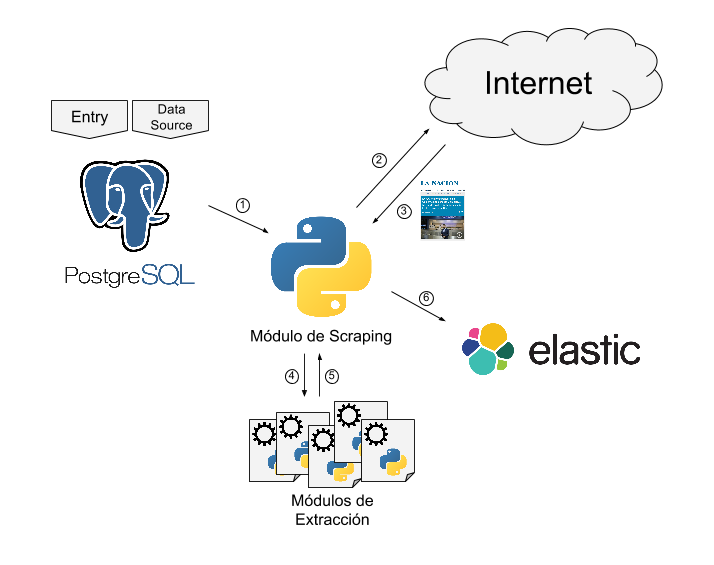
\includegraphics[width=\textwidth]{images/diag-corpus-autoscraper}
  \caption{\textit{Arquitectura general del sistema construido.} El módulo de scraping toma los datos de la
base de datos (PostgreSQL), descarga la página web de Internet y se lo envía al módulo de extracción
adecuado, guardándolo finalmente ya procesado en Elasticsearch.}
  \label{fig:autoscraper-arq}
\end{figure}

A continuación detallaremos cada uno de estos componentes.


\paragraph{Modelo de Datos}

El modelo de datos consiste de fuentes de datos (\texttt{DataSource}) y de entradas
(\texttt{Entry}), almacenados en una base de datos \textit{PostgreSQL}~\cite{PostgreSQL}. Los
\texttt{DataSource} son un modelo simple que describe las fuentes de palabras registradas en el
sistema y cuenta básicamente del dominio del sitio (e.g. \texttt{lanacion.com.ar}), con el que se
identifica a la fuente. Además mantiene dos atributos adicionales: si está activo (esto es, si se
tienen que extraer documentos del mismo), y el nivel de concurrencia con el cuál realizar pedidos
(para no saturar a la fuente; su funcionamiento se detalla más adelante).

Por otro lado, las \texttt{Entry} son registros que identifican cada documento de cada fuente de
palabras, junto con el identificador a nivel de dicha fuente, el resultado del proceso de
extracción, la fecha en la que se agregó, el último intento, la cantidad de intentos, y la fuente a
la que pertenece. El resultado del proceso puede ser \textit{pendiente}, cuando todavía no se
intentó descargar el artículo asociado, \textit{éxito}, cuando se extrajo correctamente el
contenido, o uno de tres indicadores de error (\textit{no encontrado}, \textit{imposible de
procesar}, o \textit{intento fallido}, que se describen más adelante). Con la cantidad de intentos
se busca evitar que un artículo no se descargue por un error incidental, buscando reintentar hasta
cinco veces dicha acción.

Así, es posible mantener un registro detallado y estadísticas de todo el proceso de extracción. Para
cada fuente de datos, es posible saber cuántas entradas fueron revisadas, qué porcentaje de éstas no
contienen un documento asociado, y si alguna fuente está teniendo problemas en la extracción. Esto
último ayuda, por ejemplo, a detectar rápidamente un cambio de diseño en un sitio que provoque que
las reglas XPath queden obsoletas.


\paragraph{Módulos de Extracción}

Los módulos de extracción describen cómo es la interacción con los sitios de noticias en tres
aspectos: en cómo obtener la lista de identificadores que faltan procesar, en cómo obtener el
contenido de un artículo dado su código HTML, y en cómo obtener metadatos adicionales del artículo
(como su fecha de publicación). Para ello se define una interfaz que cada módulo debe implementar,
consistente de los siguientes elementos:

\begin{itemize}

\item Constantes \texttt{SOURCE\_DOMAIN} y \texttt{DOCUMENT\_URL}, que especifican el nombre de la
fuente (e.g. \textit{lanacion.com.ar}) y la URL de sus documentos dado un identificador,
respectivamente.

\item Función \texttt{get\_missing\_ids}, que recibe una lista de identificadores ya existentes en la
base de datos y devuelve los identificadores faltantes. Para esto la función puede, por ejemplo,
entrar a la página inicial del portal y obtener el identificador asociado a la noticia más reciente.

\item Función \texttt{get\_content}, que recibe la respuesta del portal ante el pedido de un artículo
particular. Esta función deberá revisar el código de respuesta para asegurarse que efectivamente se
haya encontrado un artículo. Aquí se encapsula la lógica de extracción del texto limpio, ya sea
mediante la utilización de reglas XPath o selectores CSS, mediante la ayuda de la biblioteca
\texttt{lxml}~\cite{LXML}. En caso de tener éxito, devolverá el contenido del artículo y un valor de
salida \texttt{success}; en caso de haber un error, devolverá \texttt{notfound}, \texttt{failure}, o
\texttt{unparseable}. El objetivo de esta distinción es saber si es necesario reintentar porque el
fallo fue por un error circunstancial (caso \texttt{failure}), si no existe un artículo (caso
\texttt{notfound}), o si hubo un problema al extraer los datos (caso \texttt{unparseable}), en cuyo
caso será necesario revisar el proceso de extracción.

\item Función \texttt{get\_metadata}, que recibe la respuesta de un artículo para el cual se extrajo
exitosamente el contenido, y devuelve los metadatos pertinentes al documento (fecha de publicación,
título, etc.).

\end{itemize}

Así, es posible incorporar una nueva fuente de palabras simplemente agregando un archivo Python que
siga la anterior interfaz. El módulo de scraping se encargará así de dar de alta la nueva fuente en
la base de datos y empezar a descargar el contenido. Esto brinda un diseño flexible y fácil de
extender en un futuro.


\paragraph{Módulo de Scraping}

El sistema corre como un \textit{daemon} que realiza el siguiente ciclo:

\begin{itemize}

\item Revisa cuáles son las fuentes de datos existentes, junto a su configuración, dando de alta en
la base de datos cualquier fuente que no tenga un registro, en base a los módulos existentes.

\item Para cada fuente de datos, crea las entradas faltantes en la tabla correspondiente, en base a
lo que le indique el módulo de extracción asociado a la fuente.

\item Para cada entrada cuyo estado es \textit{pendiente}, se descarga el HTML del artículo asociado
y se extrae tanto el contenido como los metadatos del mismo, de acuerdo a lo especificado en el
módulo de extracción asociado a la fuente.

\item Se actualiza la entrada con el resultado obtenido, y se almacena el documento extraído en
Elasticsearch con el formato adecuado.

\item Cuando no quedan más entradas pendientes, duerme por 15 minutos y vuelve a empezar el ciclo.

\end{itemize}

Con el fin de no tener que esperar por las respuestas de los sitios de noticias uno a uno, lo que
implicaría una espera de décimas de segundos para cada documento que haría imposible la descarga de
los millones que se requieren, el módulo de scraping se implementa como un bucle de eventos.

Un bucle de eventos (\textit{event loop}, en inglés), es una construcción que permite ejecutar
concurrentemente funciones que dependen de eventos externos bloqueantes (como acceso a un
dispositivo de Entrada/Salida) sin que el hilo del programa principal tenga que bloquearse
esperando, de manera similar a como hace un sistema operativo de tiempo compartido.

Ésta técnica consiste de un bucle principal que se encarga de ejecutar una serie de corrutinas, las
cuales se suspenderán cuando sean bloqueadas esperando un evento externo y continuarán su ejecución
cuando el bucle principal se lo indique. Para esto, el bucle debe emplear técnicas de
\textit{polling} (o la funcionalidad equivalente que provea el sistema operativo) para saber cuándo
un evento está listo para ser atendido.

Se utilizó la implementación de la biblioteca estándar de Python de esta construcción, denominada
\texttt{asyncio}~\cite{Asyncio}. De esta forma, es posible descargar cientos de artículos
concurrentemente, sin demorarse por un sitio particularmente lento. Para ello, cuando se recorren
las entradas pendientes y se realiza un pedido HTTP para obtener el artículo, la función que procesa
los artículos se suspende hasta que la descarga finalice, continuando con otro artículo mientras
tanto.

De todos modos, es necesario limitar la cantidad máxima de concurrencia por dos razones: primero,
porque se corre el riesgo de iniciar miles o hasta millones de pedidos en simultáneo, lo cuál es
computacionalmente muy costoso e improductivo; y segundo, porque no se quiere saturar a los sitios
de noticias con demasiados pedidos activos, ya que se correría el riesgo de que se le prohiba el
acceso a nuestro sistema. Algunos sitios son particularmente susceptibles a este último punto, por
lo que se decidió que el nivel de concurrencia sea configurable a nivel de cada fuente de datos.

Para concluir esta sección, presentamos algunos números del proceso. Mediante este sistema se
extrajeron $11.363.251$ documentos de 20 portales de noticias, obteniendo así un total de
$4.391.944.678$ palabras. Se dieron de alta un total de $17.053.703$ entradas, de las cuales
un $58,6\%$ llevó a la extracción exitosa de un documento, donde algunas fuentes de noticias
fueron más rentables que otras.


\subsubsection{Scraping Manual}

\paragraph{Scrapy}

Para las fuentes de palabras que carecen de una estructura que favorece su extracción automática
mediante el método anterior, se utilizaron también técnicas de scraping convencionales, a través de
\textit{Scrapy}~\cite{Scrapy}.

Scrapy es un framework escrito en Python ideado para brindar una solución integral al problema de
realizar scraping en la web. Entre sus principales ventajas se encuentra la sencillez de su
propuesta, basada en la construcción de web spiders (arañas web) especializadas para cada dominio
del cual interesa extraer información. Además, Scrapy brinda una serie de herramientas y utilidades
que simplifican de manera importante este tipo de tareas.

La habilidad de recorrer el contenido de un portal iterando sobre los identificadores de sus artículos
o noticias es una gran ventaja y facilita mucho el trabajo de extracción, pero hay multitud de fuentes
interesantes que no permiten esta metodología. En particular los portales El País (tanto de Madrid
como de Uruguay) son de sumo interés para la construcción del corpus del proyecto y se requirió
construir web spiders para los mismos.

Para este tipo de casos se escribieron web spiders con Scrapy que primero navegaran a las
secciones de archivo o hemeroteca de cada portal y que luego, siguiendo diferentes pasos,
accedieran a los artículos en sí mismos. Naturalmente, las rutas de navegación para cada sitio
son variables y por lo tanto fue necesario escribir spiders para cada portal que requiriera
scraping manual. Es importante mencionar que cada uno de estos spiders especializados cuenta
con reglas específicas para extraer y limpiar el contenido útil de cada artículo extraído.

Una vez construido, cada web spider es ejecutado para agregar los artículos recopilados al corpus.
Cada uno de ellos puede ejecutarse en varias oportunidades, permitiendo obtener nuevos artículos y
parando cuando se detecta que ya se obtuvieron todos los nuevos resultados. Además, en todos
los casos se buscó encontrar identificadores únicos para cada artículo de forma de no agregar
elementos repetidos al corpus. Esto se logró utilizando identificadores propios de cada portal o usando
fragmentos de la URL de cada artículo.

\paragraph{Scripts de limpieza}

Para algunas fuentes, como es el caso de Wikipedia, se puede descargar su contenido directamente
a través de un dump (o volcado) en algún formato portable y de fácil distribución. Por ejemplo, en
algunos casos puede descargarse un dump de una base de datos en formato SQL, o también en
formato XML, como es el caso de Wikipedia. Otra fuentes utilizan sus propios formatos para la
distribución de sus datos, pero en todos ellos resulta indispensable realizar una limpieza antes
de proceder a agregarlos al corpus.

En nuestro caso, para aquellas fuente que ofrecen su contenido de forma directa y sin necesidad
de realizar scraping, decidimos utilizar scripts de limpieza escritos en Python que lidien directamente
con los dumps obtenidos. Los mismos recorren todos los archivos que compongan un dump en
particular, extrayendo y limpiando los datos útiles para luego indexarlos directamente en Elasticsearch.

El proceso de extracción resulta más o menos complicado dependiendo del formato provisto por cada
fuente, pero las tareas de limpieza suelen ser sencillas. El objetivo siempre es preservar el texto
original, limitándonos simplemente a remover etiquetas o restos de código que pueden quedar al
procesar los documentos.

En particular, para Wikipedia se utilizó el popular script WikiExtractor~\cite{WikiExtractor}, para las
tareas más complejas de procesamiento del dump de Wikipedia, junto con un script propio para el procesamiento
final y posterior inserción en Elasticsearch. Dicho script se encuentra en el archivo \texttt{wiki.py},
en el directorio \texttt{scripts} del código fuente del proyecto. Se utilizaron también scripts para la
limpieza e inserción de las sesiones del parlamento Uruguayo (\texttt{parlamento.py}) y los documentos
oficiales de las Naciones Unidas (\texttt{multiun.py}). Finalmente, para las fuentes EU Bookshop y el
sitio \textit{tusubtitulo.com} se utilizaron los scripts \texttt{eubookshop.py} y \texttt{tusubtitulo.py}
respectivamente.


\section{Resultado}

En esta sección se pretende presentar un análisis de la composición y la calidad del corpus
construido, mostrando algunas cifras por vertical de texto. Se incluye una caracterización del
corpus según los tipos de fuente que lo componen y se presenta una breve discusión acerca de los
aspectos más importantes de calidad.


\subsection{Composición del Corpus}

Luego de meses de trabajo se logró no solo alcanzar la meta de dos mil millones de palabras,
fijada al inicio del proyecto, sino que se logró superarla ampliamente logrando construir un
corpus con casi seis mil millones de palabras ($5.970.953.659$). Esta cantidad se encuentra
repartida en trece millones de documentos ($13.108.394$), con un promedio de 455 palabras
por documento.

La cantidad total de palabras alcanzada en el corpus es un logro sumamente significativo,
consiguiendo casi triplicar la cantidad fijada como objetivo al comienzo del proyecto. Este hecho
adquiere mayor relevancia considerando que los mayores tamaños conseguidos en los
trabajos de estado del arte en materia de construcción de corpus rondan los ocho mil
millones de palabras.

Sin embargo, es importante resaltar que todos los trabajos que alcanzaron dichas cantidades
utilizaron técnicas de crawling masivo como metodología para la construcción de sus corpus. Esto
contrasta con el enfoque adoptado en el presente proyecto, en el cuál se realizó crawling
selectivo logrando algunas garantías básicas de calidad y un conocimiento más detallado
de los documentos que componen el corpus. El objetivo fue por tanto lograr un corpus de
calidad por construcción.

Como ya se mencionó, todos los documentos que componen el corpus fueron etiquetados de
acuerdo a sus características. Las etiquetas utilizadas pueden dividirse en tres categorías:
tipo de documento, región de origen e idioma. Naturalmente, todos los textos que componen
el corpus contienen la etiqueta de idioma español, pero aun así se decidió incluir este tipo de
etiqueta pensando en un posible trabajo futuro, donde las herramientas aquí construidas podrán
ser utilizadas para trabajar con corpus en varios idiomas.

En el cuadro \ref{table:corpus_country} puede verse el detalle de cantidad de palabras por
zona geográfica de los documentos que componen el corpus, detallando además las
cantidades por tipo de documento. En el cuadro \ref{table:corpus_doc_type} en cambio, se
realiza un análisis complementario incluyendo datos sólo por tipo de documento.

\begin{table*}[h]
    \centering
    \begin{tabular}{lccc}
        \hline
        Tipo de documento & Documentos & Palabras & Proporción (palabras)\\
        \hline
        Noticias & 11.318.776 & 4.376.315.796 & 73.2\%\\
        Wikipedia & 1.113.372 & 416.932.056 & 7.0\%\\
        Documentos oficiales & 69.965 & 417.833.686 & 7.0\%\\
        Escritura amateur & 372.627 & 318.811.674 & 5.3\%\\
        Libros & 7.437 & 202.546.087 & 3.4\%\\
        Foros & 199.129 & 133.942.466 & 2.2\%\\
        Subtítulos & 27.105 & 106.501.897 & 1.8\%\\
        \hline
    \end{tabular}
    \caption{Composición del corpus por tipo de documento.}
    \label{table:corpus_doc_type}
\end{table*}

Es importante notar que no todas las fuentes lograron ser etiquetadas por su origen y que la
proporción que se muestra en el cuadro \ref{table:corpus_country} corresponde a la comparación
con la totalidad de palabras del corpus. Por otro lado, sí se logró etiquetar todos los documentos
de acuerdo a su tipo de documento.

\begin{table*}[h]
    \centering
    \begin{tabular}{llccc}
        \hline
        Origen & Tipo & Documentos & Palabras & Porcentaje\footnote{Proporción de palabras sobre el total del corpus.}\\
        \hline
        Argentina
         & Noticias & 2.130.965 & 969.052.149\\
         & Foros & 199.129 & 133.942.466\\
         & \textit{Total} & 2.330.094 & \textbf{1.102.994.615} & 18.5\%\\
        \\
        México
         & Noticias & 2.489.280 & \textbf{934.356.171} & 15.6\%\\
        \\
        Uruguay
         & Noticias & 1.961.752 & 748.998.277\\
         & Docs. oficiales & 3.418 & 103.988.021\\
         & \textit{Total} & 1.965.170 & \textbf{852.986.298} & 14.3\%\\
        \\
        España
         & Noticias & 1.631.521 & \textbf{809.067.269} & 13.5\%\\
        \\
        Paraguay
         & Noticias & 1.919.737 & \textbf{529.593.496} & 8.9\%\\
        \\
        Unión Europea
         & Docs. oficiales & 66.547 & 313.845.665\\
         & Libros & 7.437 & 202.546.087\\
         & \textit{Total} & 73.984 & \textbf{516.391.752} & 8.6\%\\
        \\
        Chile
         & Noticias & 713.541 & \textbf{228.490.971} & 3.8\%\\
        \\
        Perú
         & Noticias & 313.081 & \textbf{100.124.272} & 1.7\%\\
        \\
        Bolivia
         & Noticias & 158.924 & \textbf{56.640.181} & 0.9\%\\
        \hline
    \end{tabular}
    \caption{Composición del corpus por zona geográfica.}
    \label{table:corpus_country}
\end{table*}

Como se puede ver, la mayor cantidad de palabras provienen de fuentes del tipo noticias,
aunque de todas formas se consiguió el objetivo de tener una considerable variedad de
tipos de fuentes representadas.


\subsection{Calidad del Corpus}

Como ya se comentó previamente, al momento de elegir las fuentes para la composición
del corpus se realizó un cuidadoso proceso de selección. Para las fuentes que requirieron
crawling se escribieron reglas específicas para obtener el contenido útil de sus páginas. En
el caso de fuentes recopiladas en formatos disponibles para descargar de forma directa, se
escribieron scripts de limpieza especializados para cada una. De esta forma, se buscó en
todo momento que el corpus generado tuviera atributos de calidad por construcción.

En casos donde se requiere un corpus etiquetado, los requerimientos de calidad del mismo
son naturalmente más exigentes y es recomendable realizar un análisis riguroso de sus
características de composición y calidad. Sin embargo, para nuestro caso de estudio
consideramos como suficientes los atributos de calidad obtenidos gracias a las técnicas
utilizadas para la construcción del mismo. Todas las reglas de extracción y scripts de
limpieza fueron debidamente evaluados de modo de obtener una alta confianza en la calidad
de la composición del corpus.
